\documentclass[12pt,a4paper,twoside,titlepage,headsepline,numbers=noenddot,listof=totoc,index=totoc,bibliography=totoc]{scrartcl}


\ifx\pdfoutput\undefined
\pdffalse % we are not running pdflatex
\else
\pdfoutput=1 % we are running pdflatex
\pdfcompresslevel=9     % compression level for text and image;
\usepackage[pdftex,bookmarks=true,bookmarksopen=false,bookmarksnumbered=true,linktocpage,colorlinks=true,backref,pagebackref, linkcolor=black,  citecolor=black, urlcolor=black]{hyperref}
\usepackage[pdftex]{graphicx}
\usepackage{microtype}
\fi

\usepackage{amsfonts}
\usepackage{algorithmic}
\usepackage{url}
\usepackage{color}
\usepackage{tabularx}
\usepackage[T1]{fontenc}
\usepackage[utf8x]{inputenc}
\usepackage{textcomp}
\usepackage{bbm}
\usepackage{marvosym}
\usepackage{amsmath}
\usepackage{amssymb}
\usepackage{ntheorem}
\usepackage{fancyvrb}
\usepackage{subfigure}
\usepackage{mathptmx} 
\usepackage[scaled=.90]{helvet} 
\usepackage{courier}
\usepackage[rightcaption]{sidecap}
\usepackage{lscape}
\usepackage{supertabular}
\usepackage{everysel}

\RequirePackage{xspace}

\setcounter{secnumdepth}{3}

\newcommand{\p}[1]{\texttt{\small #1}}

\theoremstyle{break}
\newtheorem{defi}{Definition}[section] 
\newtheorem{bsp}{Beispiel}[section] 

\definecolor{gray}{gray}{0.95}
\setlength{\fboxrule}{2pt}

\providecommand{\ext}[1]{}
\providecommand{\TODO}[1]{{\small ~\\\hrule\vspace{0.1cm}\hrule~\\\textbf{TODO}:  #1~\\\hrule\vspace{0.1cm}\hrule~\\}}

\pagestyle{headings}

\begin{document}                

% ************************************************************
% *****                    Titelseite                    *****
% ************************************************************

\setcounter{page}{1}
\pagenumbering{Roman}

\begin{titlepage}
\thispagestyle{empty}
\begin{center}

		
\includegraphics[width=12cm]{figures/uni-logo}\\
                     
  \vspace{4cm}
		{\LARGE  \textbf{Report}} \\ 
		\vspace{0.5cm}
		{\Large IMT4888 Specialisation in Game Technology (2017 Fall) } \\ 
		\vspace{1.5cm}
		{\Large\textbf{Magic Sand Buggy}} \\
		\vspace{0.5cm}
		Gjøvik, 16/11/2017 \\
		\vspace{2cm}
		\textbf{Jan Tiemann} 			
\end{center}
\end{titlepage}

\clearpage
	
%\thispagestyle{empty}

%\tableofcontents

%\clearpage

\pagenumbering{arabic}
\setcounter{page}{1}

% ************************************************************
% *****                    Inhalt                        *****
% ************************************************************

\tableofcontents
\newpage

\section{Introduction}
This is a report about my project work in the course IMT4888 Specialisation in Game Technology. I have never written a report like this in my study career before and I hope I meet the expectations. 

The aim of this project was to build upon the results of Skotvold, Somby, M´Hamed, Lecoq and extend it to a full multi-player Virtual Reality(VR) / real sandbox game. The main vision was a cooperative racing game with a changing racetrack. One player is in VR driving a car around in a landscape. The landscape is based of the height profile of a real world sandbox. Another player or a group of players are at the sandbox and manipulate the sand. Changes in the real world sand are reflected by the in-game landscape at runtime. The position of the car and other race track elements along with the height profile are projected onto the sand. The aim of the game is to allow the driver to perform specific maneuvers. For example, if the current objective is to jump a long distance. The sandbox players have to form a hill with a long enough runway in-front of it to allow the driving player jump with enough speed off the hill.  

Because of lacking manpower and changes in the underlying technology only a proof-of-concept could be realized.

\subsection{Sandbox Applications}
The foundation for this and the previous project was the Augmented Reality (AR) Sandbox created by researchers at UC Davis\footnote{\url{https://arsandbox.ucdavis.edu}}. The later used Software \textit{Magic Sand}, which is a partial port of the \textit{AR Sandbox} to the \textit{openframeworks} framework, was mainly written by Thomas Wolf\footnote{\url{https://github.com/thomwolf/Magic-Sand}}. Both use the same setup. A Microsoft \textit{Kinect} and a projector are installed over a sandbox and face the sand surface. The depth sensors of the \textit{Kinect} allow the application to scan the height of the surface. Afterwards, the projector is used to display this height map back on the sand. Extensive calibration between \textit{Kinect} depth image and back projection is needed to align the projection with the sand surface. 

The internal code structure of the \textit{AR Sandbox} project was very opaque and made creating extensions difficult. Individual lines of code were commented but the architecture was not clear and the application was not consistently modularized. It felt like a further developed prototype. At 1/3 of the project time the alternative \textit{Magic Sand} was found and a switch was made. \textit{Magic Sand} was very well modularized. In addition to that, it was build on top of the \textit{openframeworks} framework which made OS-transparent development and preparing the build environment easier. 


\subsection{Previous Work}
The previous work was created for the fulfillment of a bachelor level course's requirement. It consisted of two modules. One server which was an extension to the \textit{AR Sandbox} and a demo client application which was build with the Unity Engine. The server extracted the height map from the \textit{AR Sandbox} and send it upon a request from the client over an TCP connection. The client rendered the height map by sculpting a plane accordingly. The transaction used a simple protocol which employed packets with a short header and a payload tail. To serialize the height map, the float values were truncated to three digits, converted to strings using the actual number chars and then send as ASCII chars over the network.  Additionally the client employed meshes without updated colliders to present the height data. However, those colliders are essential if one wants to drive with something on it. The most important contribution to the current  project was to locate where it was possible to extract the height data from \textit{AR Sandbox}. This had to be a quite hard task since the quality of the code structure was lacking, as mentioned before. 

When the setup was switched from \textit{AR Sandbox} to \textit{Magic Sand}, I decided to abandon the previous project and write my own implementation. I had to do that for the unity party anyway and it would have been more work to understand the existing server and adapt it to \textit{Magic Sand} that to write it anew. Furthermore \textit{openframeworks} offered an TCP server implementation so half of the server was already done. I kept the general protocol structure but more on that in chapter \ref{ch:protocol}.


\section{Method and Results}
The project had the same structure as the previous one. It was split into client and server. The server was an extension to the sandbox software with the main task of extracting and sending the height data. In addition to that, the server had to receive and render the position of the car back onto the sand in this project. The client had to request height data, sculpt terrain according to it, take user inputs, run a racing game and send the position of the car back to the server.


\subsection{Server}
As mentioned before was the server an extra module of the sandbox application. It fit into the structure just like some of the games which were already implemented. It used the offered facilities of the \textit{Magic Sand} software without requiring any changes to the core functionality of the application. As the base software was written in C++ the server was written in C++, too.

The height data was extracted from a filtered image of the \textit{Kinect} depth sensors. The filtering was done by \textit{Magic Sand}. After some testing it was obvious that the data was wrong by a non constant offset. Besides the height height image, the used facility offered a base plane equation. If this base plane was added to the data the offset vanished and the rendered surface resembled the actual sand surface. Sadly, it was not clear in which range the values of the height map and base plane resided in. But I guessed and scaled the baseplane height by half of its offset and the results looked very accurate. (see Figure \ref{fig:sandboxheightshade})

The projection of the car on the sand surface was done alike to the drawing of fishes and rabbits of one of the pre-implemented games. Thanks to the good structure of \textit{Magic Sand} it was easy to learn how it was done and easy to adapt to my use. Currently, the player's car is represented by a simple dot. But I am very confident that this can be easily extended to a vector drawing or even sprite using \textit{openframeworks} capabilities. 

In addition to the actual server a dummy server was build. It is basically a standalone version of the actual server and serves a simple $sin$ wave patter which changes over time. First it was used to test the, later explained, protocol. After the transaction were stable, it allowed me to continue the development of the client independent of the sandbox. Another reason for the relatively high maturity of this dummy application was that the idea of a sandbox game jam was considered. At such an event, not every team would have constant access to the sandbox but it still needs something to test their code against.

\TODO{picture of dummy server out put}
\TODO{picture of offset error}

\begin{figure}
	\centering
	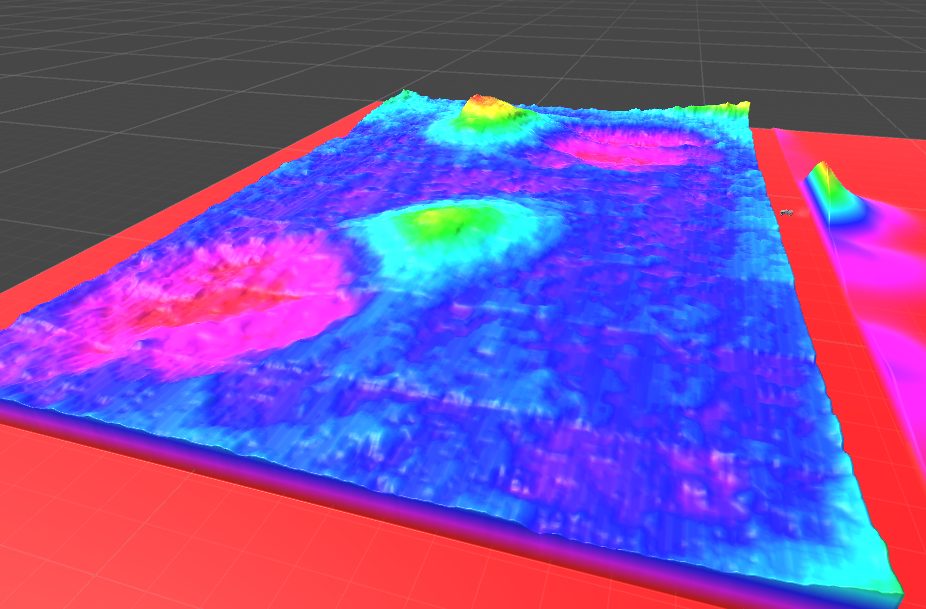
\includegraphics[width=0.8\linewidth]{figures/sandboxHeightShade}
	\caption{Rendered height map on the client using a height color shader. The vertical lines in the terrain are an artifact of the sandbox application, possibly cause by the too low resolution of the \textit{Kinnect}.}
	\label{fig:sandboxheightshade}
\end{figure}

\subsection{Client}
The client is written in c\# and uses the \textit{Unity} engine. For the network capabilities standard library \textit{.NET} TCP functionality was used. Initially it was planed to use the \textit{Unreal} engine. However, it was not possible to modify terrain at runtime with it. \textit{Unity}, on the other hand, implemented this feature may versions ago. 

\textit{Unreal}s example vehicle implementation was more usable for this scenario since it was a sand buggy and served as inspiration for the project name. But because of the previous mentioned reason \textit{Unity} had to be used and with it its example vehicle implementation. Unfortunately, this was a street car with skid mark animations and screeching sounds. Consequently, the driving performance on the bumpy sand surface was poor. A lift of the car's body and colliders along with an increase in the range of the wheel's suspension improved that performance to acceptable levels. (also see Figure \ref{fig:streetcarbuggy}) There was not enough time/manpower to build proper car physics.   

\begin{figure}
	\centering
	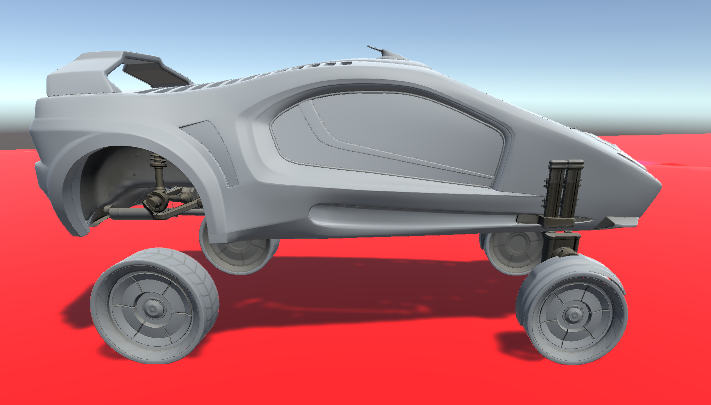
\includegraphics[width=0.7\linewidth]{figures/streetcarbuggy}
	\caption{\textit{Unity}'s demo car adjusted for desert use.}
	\label{fig:streetcarbuggy}
\end{figure}

To improve the driving experience further the sand terrain was smoothed by a simple median filter. In the same step the region around the car was protected from change. This was done to avoid having an update move the terrain which was under the car above it and causing the car to fall through the map.

Other filters which could be turned on allowed to reduce heights which were at the maximum level and scale the height map to the full range. In the early phases of the project the sand surface was not as pronounced as desired. This was especially true since the base plane offset error (mentioned in the previous chapter) was not discovered. To counter this, I introduced a filter that measured the highest and lowest point in the height map and scaled the map in such a way that those points resided at the highest and lowest point possible of the terrain object. Initially, this worked not as desired since everything that was out of \textit{Magic Sand}'s region of interest was set to the highest value. Reducing those values allowed the rescaling to achieve the desired effect. However, caution needed to applied since setting those values to zero simply would have turned the problem on its head. 

After the offset error was discovered and fixed, those filters were less needed. But still they help to produce more pronounced looking landscapes. Later it turned out that they are unsuited for use in an actual game scenario. During the game the height of the lowest and highest points change constantly and, even worse, sometimes the body parts of the sandbox players are recognized as high height parts of the sand surface thereby the scaling is constantly changing and the rendered surface feels very unstable for the driving player.

\TODO{pictures of (un)scaled/nulled}

For a proof-of-concept back-projection which will be later discussed in chapter \ref{ch:backProjection} a height color shader hat to be implemented. The height of the terrain was used as hue value of a color in the HSL color model. This color was then translated to RGB and used to paint the corresponding point on the terrain texture. An example can be seen in figure \ref{fig:sandboxheightshade}.

To test the game in VR, the VR assets were downloaded from the \textit{Unity Asset Store} and put into the game. They worked without an issue and allowed to take a first glimpse of how a finished game may look. 
 

\subsection{Protocol}
\label{ch:protocol}
The used protocol to transmit the height map were an adaptation of the one used in the previous work. But instead of sending chars of digits the full range of a byte was used and the header shrunk to a single leading byte. In addition to that there was a similar protocol for the transmission of the player's car position.  
Both protocols only support maps of the size 640 times 480 pixel/units.

\subsubsection{Height Map Protocol}
To request map data from the server the client sends a single byte, called leading byte in the code comments, containing the number "2" at port 9966 over TCP. Upon receiving this byte, the server transforms the float height values of the height map into the range 0 to 255. Now fitting into a byte, the height values are send row by row over the network. On the other end, the client receives the values, puts the map together and processes it. 

Since nearly only raw data is send over the network each request cost only $640*480b+1b=300kb$ payload data. Using a powerful linux mint machine as server, my 2-physical-cored Laptop as client and wifi I was able to see changes in the sand in nearly real time. Therefore, I did not conducted a further analysis of the transmission times. For the game this speed is even problematic since heads or arms of the sandbox players, while they are sculpting the sand, are transmitted to the client and rendered into the sand. Thereby, very suddenly appearing, steep and high hills are created which may confuse the driving player.

In addition the the height map request the server may echo a message for debug purposes. A 256 byte long ASCII message preceded by a byte with "1" encoded in it will be returned without the leading byte if the server works correctly.

\subsubsection{Car Position Protocol}
As time was running out this protocol is a fast copy of the previous one. Port 9967 is used to allow transmission of map data and updates of the car's position simultaneously. The client sends every 500ms five bytes containing the cars position preceded by a byte with "2". As I did not want to bother with sizes of integer and floats between linux, windows, c++ and c\# and endian conventions of the underlying frameworks \textit{.NET} and \textit{openframeworks} I simply encoded the position values as the sums of three or two bytes. I had already created functionality which got me the players position projected into height map texture coordinates. So I got x coordinates ranging from 0 to 640 and y coordinates ranging from 0 to 480. In the message the x value is sum of the first thee bytes, thereby having a possible range of 0 to $255*3=765$, and the y value is the sum of the last two values with a range from 0 to $255*2=510$.

\subsection{Repositories}
All modules used \textit{git} as version control. The servers are \textit{openframeorks} apps and need to be put in the corresponding folder to work correctly.

\begin{itemize}
	\item The \textit{git} repository of the server can be found at:\\ \url{https://github.com/moreApi/Magic-Sand-Buggy}
	\item The \textit{git} repository of the dummy server can be found at:\\ \url{https://github.com/moreApi/OfServerTest}
	\item The \textit{git} repository of the client (and this report) can be found at:\\ \url{https://github.com/moreApi/MagicSandBuggyUnity}
\end{itemize}

\section{Discussion}
In my personal opinion I would say that this project went quite well considering the mid-development technology change, the resulting inusability of the previous work and consequent rewrite of it and the fact that it was a single person project. Nonetheless I would also say, that the switch to \textit{Magic Sand} was a smart move, because the continued work with \textit{AR Sandbox} would have not be beneficial to the project's progress and my mental health. 

As the time of writing the project is a working proof-of-concept of a multiplayer sand/VR game. Changes of the real world sand in the sandbox are reflected by the in-game sand in nearly real time. The VR player is able to drive around on the sand and the sandbox players can see the cars position in the sandbox. Actual gameplay besides this free driving is not implemented.  

\subsection{Improvements}
Most of the actual game features were implemented in the last three weeks before the hand-in. I would assume that if the deadline would have been a week or month later the project would have matured over the proof-of-concept status. Then again, students are notoriously bad at time management and I probably would reach the same result but a week later. However, I still have to do a Feature Jam for another course and I plan to do it on this project. Therefore, I compiled a short list of features and improvements I think are worthwhile to look into whether by me or someone else: 

\begin{description}
	\item[Back-Projection] Currently the information flow from the client to the server is very rudimentary. Only the car's position is transmitted and presented. This needs to be addressed. A detailed discussion of this will be conducted in the next chapter. 
	
	\item[Car Graphic] Depending on the chosen back-projection method the server stays responsible for the drawing of the car's position on the real sandbox. Currently this is done by rendering a colored dot  at the position. As mentioned before this should be improved using \textit{openframeworks} capabilities e.g. by using a sprite or a simple vector drawing.
	
	\item[Car Physics] The current car physics are based on a lifted street car. Values like weight and bouncyness need to be adjusted to get a fun dune buggy driving experience. The vehicle example from the \textit{Unreal} engine might serve as an example.
	
	\item[Actual Gameplay] For this project to be called a game actual gameplay needs to be implemented. The current sandbox experience (both meanings intended) hardly qualifies as a game experience, at least for the driving player. The sandbox players still have a sandbox to play around in, no matter what happens on the digital side. Features like pickups, objectives or racetrack generation may facilitate a better game experience.
	
	\item[Sand Movement Smoothing/Hiding] At the current state the change of the sand surface on the client happens in a very jerky and sudden fashion. Also short-lived spikes in the surface like the erroneous detection of the sandbox player's body parts as the sand surface are rendered in full. This could be avoided if the changes are applied gradually. Only a small part of the delta height between the current surface and the target heights could be applied in each terrain update. This would hide sudden spikes and likely reduce the jerkiness of the transitions. Another way to hide big sand movements would be to only apply them when the targeted regions not in view. 
\end{description}

\subsection{Back-Projection}
\label{ch:backProjection}

There are several methods to get the information about the current status of the driving player onto the sandbox and to the other players, each with their own advantages and disadvantages.  

\begin{description}
	\item[Server Rendering] In this method the server also handles the display of the cars position. Because of the last-minute implementation of the back-projection feature this method was chosen. Most of the needed functionality for this was already there. A second TCP connection was opened alike to the existing one for the height data and used to transmit the position data. The rendering of the position was done on the original sandbox projection in a similar fashion as the already implemented games using existing facilities. 
	
	A serious disadvantage of this method is that every game object or stat that the sandbox players need to see has to be serialized, send over the network from one piece of code and framework which is written in c\# to another on which is written c++ and somehow rendered within the sandbox application. If the game is compromised of 50 different objects this has to be done for each. On the other hand, an important advantage is that the already calibrated projection of \textit{Magic Sand} is used for the display. Therefore, if \textit{Magic Sand} is setup, the game is automatically setup, too.
	
	\item[Unity - two Cameras] For this approach the Unity client employs two cameras and render runs. The first one is the regular one of the main camera following the car. This is what the driving player sees. In the second one a camera is used which is positioned in the same relative position over the sandbox as the real data projector. Also the sand is colored in a similar fashion as \textit{Magic Sand} would do (for example as seen in figure \ref{fig:sandboxheightshade}). Then, the images are send to the machine on which the sandbox application is running. This could be done by a video stream. On the sandbox machine the video is shown on the projector display. If everything works as intended the colored digital sand surface should align with the actual sand surface. A very hacky proof-of-concept supports this thesis. 	\TODO{picture from video}
	
	An obvious advantage of this method is that all objects which are present in the unity application are shown on the sand and to the other players. The reason why this approach was not chosen for the current version is the very high implementation difficulty. I have no experience with different render runs in \textit{Unity}. Additionally, streaming out of \textit{Unity} seems to be a rarely requested feature, Internet resources on the topic are sparse, especially if one wants to use actual video streaming like it is used for \textit{Twitch} or \textit{YouTube}. The proof-of-concept disabled the drivers camera and used display capturing to create a stream. Both are not viable option for the actual game.	
	
	\item[Unity - two Clients] Another option would be to have another \textit{Unity} client running on the sandbox machine and using \textit{Unity}'s build in networking capabilities to update the game state. Just like in the previous method the camera of the sandbox \textit{Unity} session could be placed over the virtual sand surface and the surface itself could be colored accordingly. The driving player's client would not have to be changed in this regard.
	
	The same advantage as for the previous solution holds. However, the implementation cost was to high to do it in a short time frame. I had previous experiences with \textit{Unity}'s networking functionality and was confident that this approach would get the desired results. However, I knew splitting the client in two synchronized sessions with both getting fresh height map data from the server and having different camera and rendering settings needed more time than I had available.
\end{description}

\subsection{Ethical Concerns}
vs. natural interaction (traditional sandbox), tech/advancemend allways good?

racial body issues, handicaped people

more and more technologial playground ->higher entrance borders - body, monetary issues -> more exclusive 

one against many - more drivers

\section{Conclusion}

will continue, at least for feature jam
fun project
will ask pb museum if they want sandbox


% ************************************************************
% *****                      Ende                        *****
% ************************************************************

\end{document}